On the square $\Omega = (0,1)\times (0,1)$, the graphs of the functions
\[
y = e^{x-c},\qquad c \in\mathbb{R}
\]
are given.
For which of the following sets do the curves passing through the set
cover the square?
\begin{teilaufgaben}
\item Left boundary: $\{(0,y)\mid y\in (0,1)\}$
\item Right boundary: $\{(1,y)\mid y\in (0,1)\}$
\item Bottom boundary: $\{(x,0)\mid x\in (0,1)\}$
\item Top boundary: $\{(x,1)\mid x\in (0,1)\}$
\end{teilaufgaben}

\begin{loesung}
\begin{figure}
\centering
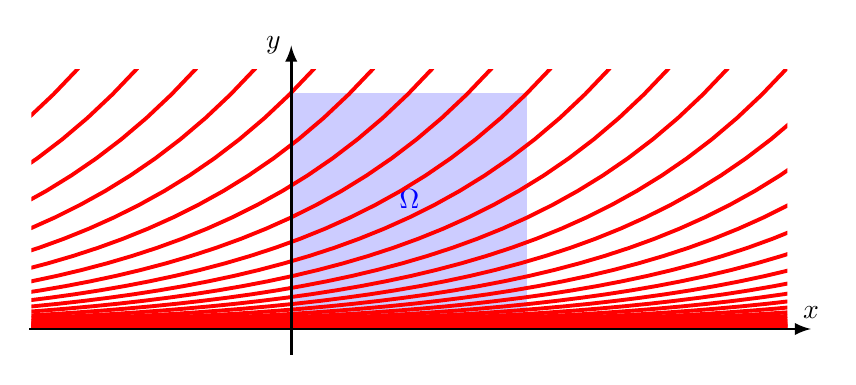
\begin{tikzpicture}[>=latex,scale=3]
\fill[color=blue!20] (0,0) rectangle (1,1);
\node[color=blue] at (0.5,0.55) {$\Omega$};
\begin{scope}
\clip (-1.1,-0.1) rectangle (2.1,1.1);
\foreach \c in {-7,-6.75,...,3}{
	\draw[color=red,line width=1.4pt]
		plot[domain={-5.1-\c}:{0.1-\c},samples=50]
			({\x},{exp(\x+\c)});
}
\end{scope}
\draw[->,line width=1pt] (-1.11,0) -- (2.20,0) coordinate[label={$x$}];
\draw[->,line width=1pt] (0,-0.11) -- (0,1.2) coordinate[label={left:$y$}];
\end{tikzpicture}
\caption{Kurven $y=e^{x-c}$ für die Fragestellungen, von welchen Teilmengen
des Randes von $\Omega$ das ganze Gebiet mit solchen Kurven überdeckt
werden kann.
\label{30000031:fig}}
\end{figure}
Die Kurven sind in Abbildung~\ref{30000031:fig} dargestellt.
\begin{teilaufgaben}
\item
The curve that passes through $(0,y_0)$ passes through
at $(x,y_0e^x)$.
So the curve starting at $(0,ye^{-x})$ passes through $(x,y)$.
But $e^{1-x}$ is $\ge 1$ so some the curve passes above
the upper right corner of the boundary.
Only the points below the curve $y=e^{1-x}$ can be covered.
\item
The curve through $(1,ye^{1-x})$ passes through $(x,y)$, so the curves
cover the square.
\item
The curve that passes through the corner $(1,1)$ is $y=e^{x-1}$, so
every point below that curve is not covered by the curves that pass
through the to boundary.
\item
Only the curve $y=0$ passes through the bottom boundary, so the curves
to not cover the square.
\end{teilaufgaben}
\end{loesung}
